\renewcommand{\theequation}{\theenumi}
\begin{enumerate}[label=\arabic*.,ref=\thesubsection.\theenumi]
\numberwithin{equation}{enumi}

\item 
Let assume that we have a point $\vec{C}\myvec{x\\0}$ which devide the linesegment $\vec{AB} $ in k:1 ratio.

\begin{align}
\myvec{x\\0} =k\myvec{1\\-5} + \myvec{-4\\5}
\\
0 = -5k + 5
\\
k= 1
\\
\vec{C} = \frac{\myvec{-3\\0}}{2} = \myvec{-1.5\\0}
\end{align}
\begin{figure}[!ht]
	\centering
	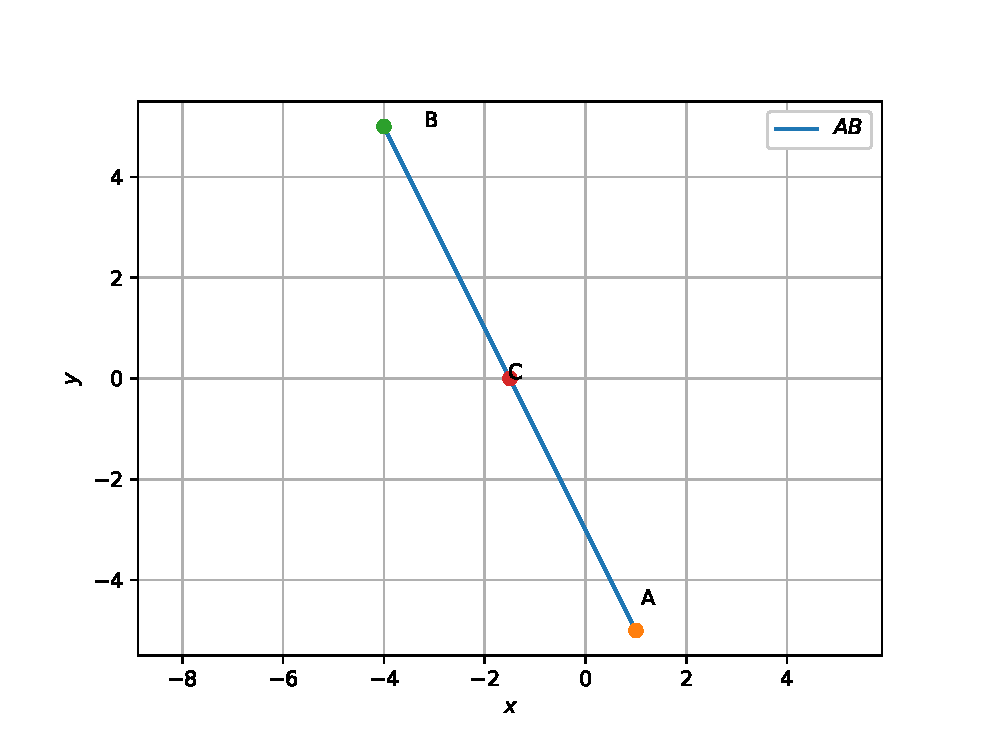
\includegraphics[width=\columnwidth]{./figures/point_on_line.eps}
	\caption{line }
	\label{fig:line}
\end{figure}
\begin{lstlisting}
codes/points_on_line.py
\end{lstlisting}

\end{enumerate}